\chapter{Funktionen}
\label{funktionen}
Abbildung \ref{Funktionen1} zeigt den Aufbau der Karteikarte \textsl{Funktionen}:
\begin{itemize}
	\item Listenfeld: Zeigt die Funktionen der Person an. 
	\item Details: 	Im Details-bereich k�nnen die Funktionen-Daten eingegeben und ver�ndert werden.
	\begin{itemize}
		\item Funktion: Funktion, die die Person aus�bt.	
		\item Organisationseinheit: Organisationseinheit in dem die Funktion g�ltig ist.
		\item Institut: In einigen Situationen ist es n�tig, dass sowohl ein Studiengang (Organisationseinheit) und ein Institut zugeordnet werden muss. 
		\item Semester: Semester in dem die Funktion g�ltig ist.
		\item Bezeichnung: Standardm�ssig wird die Bezeichnung von der Funktion �bernommen
		\item G�ltig von: Datum ab dem die Funktion g�ltig ist.
		\item G�ltig bis: Datum bis wann die Funktion g�ltig ist.
	\end{itemize}
	\item Button \textsl{Neu}: Start der Eingabe einer Funktion.
	\item Button \textsl{Loeschen}: L�schen eines markierten Eintrags.
\end{itemize}
\begin{figure}
	\centering
	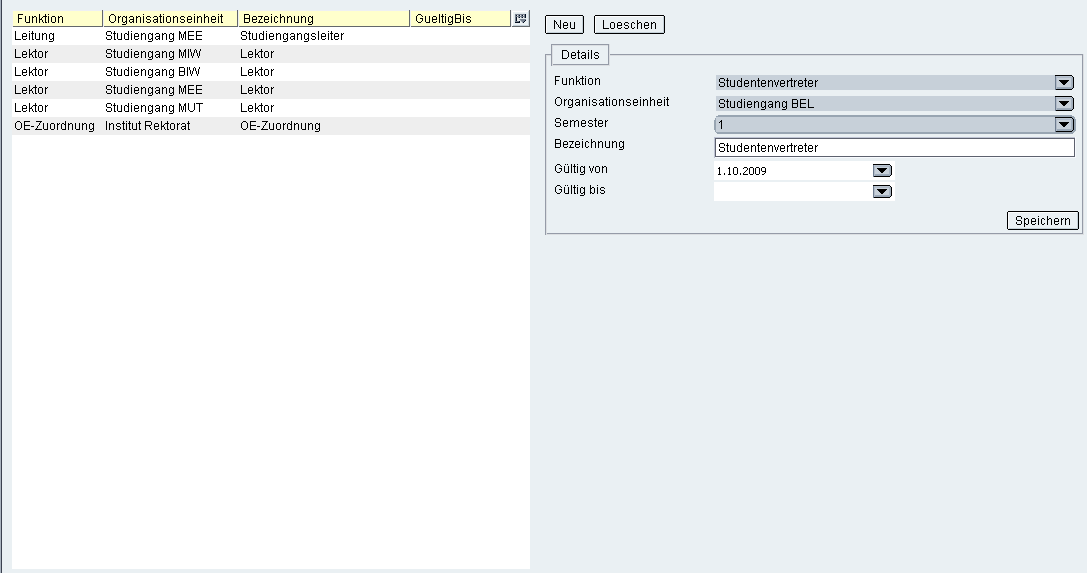
\includegraphics[width=0.75\textwidth]{FAS_Funktionen1.png}
	\caption{Die Karteikarte Funktionen}
	\label{Funktionen1}
\end{figure}
\section{Anlegen von Funktionen}
\underline{Institutsleiter eintragen:}\\
Folgende Eingaben sind vorzunehmen:
\begin{itemize}
	\item Funktion = Leitung
	\item Organisationseinheit =  Institut/Bereich, der geleitet wird.
\end{itemize}
Abschlie�end \textbf{Speichern} klicken.\\
\underline{Institutskoordinator eintragen:}\\
Es gibt 2 M�glichkeiten Koordinatoren zuzuweisen. 
\begin{itemize}
	\item 1.�ber die Lehrveranstaltung:
	\begin{itemize}
		\item F�r spezielle Lehrveranstaltungen kann ein eigener Koordinator angegeben werden. Diese werden immer Vorrangig angezeigt. Wenn zu einer LV kein Koordinator zugeteilt ist, wird jener Koordinator angezeigt der die Zuteilung �ber die Funktion hat. N�here Information unter \ref{lehrveranstaltung} (Lehrveranstaltung).
	\end{itemize}
	\item 2.�ber die Funktionen
	\begin{itemize}
		\item Funktion = Koordinator
		\item Organisationseinheit = Studiengang der Koordinatorfunktion
		\item Institut = Institut der Koordination
	\end{itemize}
\end{itemize}
\underline{OE-Zuordnung eintragen:}\\
Die Zuordnung zur Organisationseinheit wird ben�tigt um die Hierarchie der Mitarbeiter darzustellen. (Um zB die Freigaben des Urlaubes auf der CIS-Seite verwalten zu k�nnen). Wenn keine OE-Zuordnung eingetragen ist, dann werden beim Eintragen von Urlauben auf der CIS keine Freigabemails versendet.
Folgende Eingaben sind vozunemen:
\begin{itemize}
	\item Funktion = OE-Zuordnung
	\item Organisationseinheit = Organisationseinheit, der die Person zugeordnet werden soll
\end{itemize}
